\documentclass[aps,a4paper,twocolumn,showpacs]{revtex4}

\usepackage{epsfig}
\usepackage{graphicx}
\usepackage{amsmath,amssymb,color}
\usepackage{tikz-cd}
%\usepackage{stfloats}
%\usepackage[cp1251]{inputenc}
\usepackage[english]{babel}

\parskip=\medskipamount
\def\baselinestretch{1}

%---------------------------------------------------------------------

%DEFINITIONS

\newcommand{\eq}[1]{(\ref{#1})}
\newcommand{\fig}[1]{Fig.\ref{#1}}

\newcommand{\be}{\begin{equation}}
\newcommand{\ee}{\end{equation}}

\newcommand{\barr}{\begin{array}}
\newcommand{\earr}{\end{array}}

\newcommand{\beqn}{\begin{eqnarray}}
\newcommand{\eeqn}{\end{eqnarray}}

\newcommand{\bs}{\begin{subequations}}
\newcommand{\es}{\end{subequations}}

\newcommand{\bw}{\begin{widetext}}
\newcommand{\ew}{\end{widetext}}

\newcommand{\tit}{\textit}
\newcommand{\trm}{\textrm}
\newcommand{\tbf}{\textbf}
\newcommand{\mbf}{\mathbf}
\newcommand{\mcl}{\mathcal}

\newcommand\disp{\displaystyle}
\newcommand\foot{\footnotesize}
\newcommand\scri{\scriptsize}
\newcommand{\eps}{\epsilon}

\newcommand{\la}{\left<}
\newcommand{\ra}{\right>}

\newcommand{\up}{\uparrow}
\newcommand{\down}{\downarrow}
\newcommand{\lef}{\leftarrow}
\newcommand{\rig}{\rightarrow}

\newcommand{\rv}[1]{\textcolor{red}{#1}}
\newcommand{\ve}{\mathbf}


%MACRO FOR RUNNINGHEAD
\def\runninghead#1#2{\pagestyle{myheadings}
\markboth{{\protect\it{\quad #1}}\hfill} {\hfill{\protect\it{#2\quad}}}}





%---------------------------------------------------------------------


\begin{document}

\pgfdeclareimage[height=2.25cm, interpolate=true]{$P(M)$}{node_D.png}
\pgfdeclareimage[height=2.25cm, interpolate=true]{$M$}{node_L.png}
\pgfdeclareimage[height=2.25cm, interpolate=true]{$P$}{node_T.png}

\title{Reconstructing phase diagram of a non-Markovian random walk by deep learning}


\author{A.A.~Lobashev$^{1}$, S.K~Nechaev$^{2,3}$, M.V.~Tamm$^{1,4}$}

\affiliation{$^1$ Department of Applied Mathematics, MIEM, National Research University Higher School of Economics, 123458 Moscow, Russia\\ $^2$ Interdisciplinary Scientific Center Poncelet (CNRS UMI 2615), 119002 Moscow, Russia  \\ $^3$ P.N. Lebedev Physical Institute RAS, 119991 Moscow, Russia \\$^4$ Faculty of Physics, Lomonosov Moscow State University, 119992 Moscow, Russia}

\date{\today}

\begin{abstract}
Here will be an abstract
\end{abstract}

\pacs{?, ?}

\maketitle

% Introduction:
%   (1) ML is actively applied to study physics systems: models and experimental data.
\par Recently, the application of machine learning methods to various problems of statistical physics has been rapidly developing. These methods have been actively used in the study of the models of classical and quantum statistical physics \cite{phase_transitions_by_confusion, carrasquilla, ml_topological_phase_transitions, ml_quantum_phase_transitions, ml_hubbard_model, pca_and_vae_ising_model}. 

One of the problems that can be solved by such methods is the problem of determining phase transitions from an ensemble of microstates of a physical system. Because exactly solvable models are limited in their ability to describe real-world phenomena, machine learning turns out to be a useful tool for analyzing complex systems that cannot be described analytically.
%   (2) It enables to study phase transitions. These methods are often can extract order parameters by itself. Often there is a problem how to choose right order parameter.
%   (3) It is not clear how extracted phases are coincide with real thermodynamic phases.
%   (4) But it also is able to extract thermodynamic characteristics (like in Walker, 2019)
In (Walker, ICML, 2019) it was shown that deep learning models could extract features which are reminiscent of conventional thermodynamic variables. 
%   (5) % Our goal is to propose a method to construct thermodynamic order parameters and extract representations of microstate which will be invariant under the choice of microstate from the same phase. (We want a function that maps microstates into vectors encoding phases; all vectors from the same phase should be mapped into the same vector.)
Our goal is to propose a method to construct thermodynamic order parameters and extract representations of microstate which will be invariant under the choice of microstate from the same phase.
% BYOL (Bootstrap Your Own Latent, Neural Information Processing Systems, 2020) by looking at the difference between current image and average image in the batch we could learn good representations of input images.

Methods of machine learning are useful for finding regularities in big datasets of different nature \cite{???}. Recently, the application of these methods to various problems of statistical physics has been rapidly developing. One class of problems where its application seems to be fruitful is the determination of characteristics of an underlying random walk process based on individual trajectories \cite{...}. Another is the determination of a phase diagram of an equilibrium statistical physical system based on the samples of microstates at various values of parameters\cite{?}. 

From the machine learning point of view in both cases it is instructive to think of a studied model/process $S$ as rule (function, operator), which gets a relatively small set of macroscopic parameters $m \in M$ as an input and returns a vector in a very multidimensional phase space $P$, which we call \emph {microscopic state}. Importantly, this rule is probabilistic, so one can think of a microstate $\mu \in P,\ \dim(P) \gg \dim (M)$ as a function of the set of macroscopic parameters $m$ and some vector $\boldsymbol{\xi}$ of random variables, $\mu = S(m,\boldsymbol{\xi})$. By fixing macroscopic parameters we define a probability distribution on the phase space so it is convenient to associate $M$ with the corresponding space of probability distributions on $P$.

\begin{figure}[ht]
\[
\begin{tikzcd}[column sep=2em,row sep=2em]
 & \pgfuseimage{$P(M)$}  \arrow[dl, bend left = 15, "f^{-1}"] \arrow[dr, bend left = 15, "g^{-1}"] \\
\pgfuseimage{$M$} \arrow[ur,"f",  bend left = 15] \arrow[rr, bend left = 0,"h"] \arrow[rr, bend right = 25, dashed, "S", blue] && \pgfuseimage{$P$} \arrow[ul, bend left = 15, "g"]
\end{tikzcd}
\]

\caption{Relations between phase space $P$ of a physical system, space of macroscopic variables $M$ and space $\mathcal{P}(M)$ of probability distributions on $M$.}
\label{scheme}
\end{figure}

The single trajectory analysis corresponds to an inverse problem, its aim is to infer the macroscopic parameters given some set of known microscopic states, i.e., to infer $p$ given some collection of $\mu$'s. Phase classification or construction of phase diagrams is in a sense a problem of clustering: the microscopic states corresponding to the same phase are, in some respect, similar to each other, while those corresponding to different phases are different from each other. The basic idea is, therefore, is that the space $\mathbb{P}$ of parameters $p$ can be separated into a set of mutually non-intersecting domains $P_i$ (phases) so that the function $f(p,\boldsymbol{\xi})$ can be approximated by  $\bar{f}(I(p),\boldsymbol{\xi})$ where $I(p)$ is an indicator function returning the number of the phase $p$ belongs to:
\be
I(p) = i \text{ if and only if  } p\in P_i
\ee 
and the problem is to find a separation of the space $\mathbb{P}$ into phases which minimizes the difference between $f(p,\boldsymbol{\xi})$ and $\bar{f}(I(p),\boldsymbol{\xi})$. Putting it in other words, we expect that if one takes two points $p_{1,2} \in \mathbb{P}$, constructs a collection of microstates corresponding to each of them, and trains a classificator to distinguish between these microstates, then the classificator's precision will depend on whether $p_1$ and $p_2$ belong to the same phase: for the points belonging to different phases the precision will converge to unity with growing size of the learning sample, while for the points belonging to the same phase it will remain roughly $1/2$.  

Then, one might suggest a natural way to construct a phase diagram as follows \cite{Van_Nieuwenburg}. Separate the space $\mathbb{P}$ into random domains (the number of domains should be larger than the expected number of phases). Train classificator to distinguish microstates corresponding to different domains, then move domain walls randomly, train the classificator once again, and check if the new classificator has a better precision, if yes, accept the new domain wall positions. Continue this process until the domain structure allowing for a maximal possible precision of the classificator is reached. The resulting set of domains should reproduce the phase diagram. However, this algorithm is very demanding numerically, since one must retrain classificator from scratch every time the domain walls are moved. 

\par In recent years, machine learning methods have been actively used in the study of models of classical and quantum statistical physics \cite{phase_transitions_by_confusion, carrasquilla, ml_topological_phase_transitions, ml_quantum_phase_transitions, ml_hubbard_model, pca_and_vae_ising_model}. One of the problems that can be solved by such methods is the problem of determining phase transitions from an ensemble of microstates of a physical system. Because exactly solvable models are limited in their ability to describe real-world phenomena, machine learning turns out to be a useful tool for analyzing complex systems that cannot be described analytically.
\par From the point of view of machine learning, a physical system of interest can be represented as a mapping that, based on a set $\{m_1, \dots, m_K\}\in\mathcal{D}$ of macroscopic parameters of the model, generates a microstate $s$ - a certain vector in a high-dimensional space $\Omega$, and the generation process is probabilistic: the same macroscopic parameters correspond to a certain probability distribution in the microstate space. If physical system is represented by it's energy function $\mathcal{E}(s, m_1, \dots, m_K)$ then the distribution takes the form
\begin{equation}
    \mathbb{P}(s| m_1, \dots, m_K) = 
    = \frac{e^{-\mathcal{E}(s, m_1, \dots, m_K)}}{Z( m_1, \dots, m_K)}.
    \label{gibbs_distribution}
\end{equation}
where we introduced the partition function
\begin{equation}
    Z( m_1, \dots, m_K) = \int_{s \in \Omega} e^{-m\mathcal{E}(s, m_1, \dots, m_K)} d\mu(s).
    \label{partition_function}
\end{equation}
For example, in the case of the $d$-dimensional Ising model in external magnetic field, a lattice filled with $ 1 $ or $ -1 $ is constructed, which can be considered as a vector in the space of dimension $\text{dim}(\Omega)=L^{d} $, where $ L $ is the size of the lattice. Corresponding energy function is
\begin{equation}
\mathcal{E}(s, H, T) = \frac{1}{T}\left(-\sum_{<ij>}s_{i}s_{j} - H \sum_{i}s_{i}\right).
\end{equation}

\par A phase transition is a sharp change in the probability distribution $\mathbb{P}(s|m_1, \dots, m_K)$ with a smooth change in macroscopic parameters $m_1, \dots, m_K$. It is convenient to characterize such transitions in terms of regularity properties of partial derivatives of the probability  with respect to macroscopic parameters
$$
\left. \frac{\partial^{n} \mathbb{P}(s|m_1, \dots, m_K)}{\partial^{n_1}m_{1} \dots \partial^{n_K}m_{K}}\right|_{\sum_{i=1}^{K}n_i = n}
$$
Let us introduce notations
$$
\mathbb{P}(s|\bold{m}) := \mathbb{P}(s|m_1, \dots, m_K)
$$
$$
\nabla_{\bold{m}} := \left. \frac{\partial^{n}}{\partial^{n_1}m_{1} \dots \partial^{n_K}m_{K}}\right|_{\sum_{i=1}^{K}n_i = n} 
$$
Then we express partial derivatives of the probability in terms of partial derivatives of the energy and the partition function
$$
\nabla_{\bold{m}} \mathbb{P}(s|\bold{m}) = \nabla_{\bold{m}} \frac{e^{-\mathcal{E}(s, \bold{m})}}{Z(\bold{m})} =
$$
$$
= \frac{1}{Z(\bold{m})}\cdot \nabla_{\bold{m}} e^{-\mathcal{E}(s, \bold{m})} + e^{-\mathcal{E}(s, \bold{m})} \cdot \nabla_{\bold{m}} \frac{1}{Z(\bold{m})}=
$$
$$
= - \frac{e^{-\mathcal{E}(s, \bold{m})}}{Z(\bold{m})} \nabla_{\bold{m}} \mathcal{E}(s, \bold{m}) - \frac{e^{-\mathcal{E}(s, \bold{m})}}{Z(\bold{m})^{2}} \nabla_{\bold{m}}Z(\bold{m}) =
$$
$$
= - \frac{e^{-\mathcal{E}(s, \bold{m})}}{Z(\bold{m})} \left(\nabla_{\bold{m}} \mathcal{E}(s, \bold{m}) + \frac{\nabla_{\bold{m}} Z(\bold{m})}{Z(\bold{m})} \right) =
$$
$$
= - \mathbb{P}(s, \bold{m}) \cdot \nabla_{\bold{m}} \left(\mathcal{E}(s, \bold{m}) + \log Z(\bold{m}) \right).
$$
We have obtained
\begin{equation}
- \nabla_{\bold{m}} \log \mathbb{P}(s|\bold{m}) = \nabla_{\bold{m}} \left(\mathcal{E}(s, \bold{m}) + \log Z(\bold{m}) \right)
\label{regularity_of_probability}
\end{equation}
from which it is follows that all information about irregularities of partial derivatives of a canonical probability density could be characterized in terms of corresponding partial derivatives of the energy and the logarithm of partition function.

\par Usually energy of a system $\mathcal{E}(s, m_1, \dots, m_K)$ is an infinitely differentiable function of macroscopic parameters and irregularity of the partition function in \eq{partition_function} comes from integration over the phase space $\Omega$ which in the thermodynamic limit becomes infinite-dimensional. As it follows from \eq{regularity_of_probability} it is enough to consider regularity properties of partial derivatives of the logarithm of partition function
$$
\left. \frac{\partial^{n} \log Z(m_1, \dots, m_K)}{\partial^{n_1}m_{1} \dots \partial^{n_K}m_{K}}\right|_{n_1+\dots +n_K = n}.
$$
because it contains all information about phase transitions.
\par In contrasts to previous approaches to characterize phase transition using machine learning methods instead of considering canonical distribution itself \eq{gibbs_distribution} we rather consider probability distribution on the space of macroscopic parameters for a fixed microstate, by applying Bayes formula. Quantitatively, if we apply Bayes' formula to \eq{gibbs_distribution}, we obtain the probability that a fixed microstate $ s $ was generated with macroscopic parameters $ m_1, \dots, m_K $
\begin{equation}
    \mathbb{P}(m_1, \dots, m_K|s) = \frac{\mathbb{P}(s|m_1, \dots, m_K)\mathbb{P}(m_1, \dots, m_K) }{\mathbb{P}(s)}
    \label{bayes_formula}
\end{equation}
For partial derivatives we have
$$
- \nabla_{\bold{m}} \log \mathbb{P}(\bold{m}|s) = - \nabla_{\bold{m}} \log \frac{\mathbb{P}(s|\bold{m})\mathbb{P}(\bold{m})}{\mathbb{P}(s)} = 
$$
$$
= - \nabla_{\bold{m}} \left(\log \mathbb{P}(s|\bold{m}) +\log \mathbb{P}(\bold{m}) - \log \mathbb{P}(s) \right) =
$$
$$
= - \nabla_{\bold{m}} \log \mathbb{P}(s|\bold{m}) -\nabla_{\bold{m}} \log \mathbb{P}(\bold{m})
$$
Probability $\mathbb{P}(m_1, \dots, m_K)$ can be chosen to be  uniform in $K$-dimensional cube $\mathcal{D} = [m_1^{(\text{min})}, m_1^{(\text{max})}]\times \dots \times [m_K^{(\text{min})}, m_K^{(\text{max})}]$, so it's partial derivatives with respect to macroscopic parameters vanish and we have
\begin{equation}
    - \nabla_{\bold{m}} \log \mathbb{P}(\bold{m}|s) = - \nabla_{\bold{m}} \log \mathbb{P}(s|\bold{m})
    \label{rgularity_from_bayes_formula}
\end{equation}

## (0):
$$
\huge{
-\nabla_{m}\log(P(s|m)) = -\nabla_{m}\log(P(m|s))
}
$$

(1):
$$
\huge{
\mathbb{E}_{s \sim P(s|m')}[-\nabla_{m}\log(P(s|m))]|_{m = m'} = 
$$

$$
= \mathbb{E}_{s \sim P(s|m')}[-\nabla_{m}\log(P(m|s))] |_{m = m'}= 
}
$$
$$
\huge{
= \nabla_{m} ({\langle E \rangle}(m)+\log Z(m)) = \nabla_{m} ({\langle E \rangle}_{\text{eff}}(m))
}
$$

(2):
$$
\huge{
\mathbb{E}_{s \sim P(s|m')}[-\nabla_{m}\log(P(m|s))] |_{m = m'} = 
$$

$$
= \sum_{s' \in N(s); \\ s \sim P(m'|s)}[-\nabla_{m}\log(P(m|s'))] |_{m = m'} =
}
$$

(3):
$$
\huge{
 = - \nabla_{m} [\sum_{s' \in N(s); \\ s \sim P(m'|s)}\log(P(m|s')) ] |_{m = m'}
}
$$
Then full set of thermodynamic variables consists of (4):
$$
\huge{
\{{\langle E \rangle}_{\text{eff}}(a,b); \frac{\partial {\langle E \rangle}_{\text{eff}}(a,b)}{\partial a}; a; \frac{\partial {\langle E \rangle}_{\text{eff}}(a,b)}{\partial b}; b\}
}
$$

In this paper we use the machine learning methods to study the morphology diagram of a novel class of non-Markovian random walks, which is a generalization of reinforced random walks studied in \cite{sapozhnikov, ordemann1, foster} and node2vec walk used to construct vector representation of nodes on a graph \cite{grover}. We call this novel class ``random walks with volume and surface reinforcement''.

Let us first remind that reinforced random walk is a discrete-time random walk on a lattice (graph) defined in a way that the walker distinguishes between visited and unvisited cites \cite{sapozhnikov, ordemann1, ordemann2, foster} (compare also with greedy forager problem \cite{BhatRednerBenichou17}, so that, given a choice, the probability of going to an already visited site is $\exp(a)$ times larger than probability of going to a new cite, with $a$ being a parameter of the model. It is known, that for $d>1$ there is a morphological transition in this model from Brownian-motion-like trajectories at small $a$ to supercollapsed trajectories at large $a$. The visited region for a long $N$-step walk in the supercollapsed state is a compact ball linear size growing as $N^{1/(d+1)}$. Presumably, the limiting shape of this ball is spherical, although it is not proven, the thickness of its boundary is $O(1)$ with $N \to \infty$. On a 3-dimensional simple cubic lattice the transition from Brownian to supercollapsed regime occurs at $a = 1.831 \pm 0.002 $.  Note also that the $a\to -\infty$ limit of this model is the so-called true self-avoiding walk \cite{amit_parisi_peliti83}.

Here we consider a generalization of this model, which distinguishes not only steps inside and outside of the visited area, but also steps along its surface. More formally, consider a random walk on some graph $\mathcal{G}$ defined by its sets of vertices and edges $\mathcal{G} = (\mathbb{V}, \mathbb{E})$. Let $V_N$ be a set of vertices visited up to step $N$ of the walk, and $v_N$ -- the position of the walker at step $N$. For each site $v_i$, which is neighbor of $v_N$, define a weight 
\begin{equation}
    w(v_{i})=I(e_{N,i} \in \mathbb{E})\left\{
    \begin{array}{ll}
          \exp{a}, &\text{ if } v_{i} \in V_N;\\
          1, &\text { if } v_{i} \not\in V_N \text { and } v_N \text{ is the only} \\ &\text {neighbor of } v_i \text{ from } V_N ;\\
          \exp{b},&\text { if } v_{i} \not\in V_N \text { and there are } \\&\text{other neighbors of } v_i \text{ in } V_N,
    \end{array} 
\right.
\end{equation}
where $e_{N,i}$ denotes the edge connecting $v_N$ and $v_i$, and $I$ is the indicator function. Now the probability of a walker going from $v_N$ to $v_i$ on step $N+1$ is proportional to $w(v_i)$:
\begin{equation}
    P(v_{N+1} = v_{i}) = 
        \frac{w(v_{i})}{\sum_k w(v_{k})}
\end{equation}
Importantly, the walks with volume and surface reinforcement defined in this way are substantially non-Markovian, with probabilities of each new step depending on the whole history of the walk. Depending on $a$ and $b$ the trajectories of the walks exhibit several distinct morphologies, including those of Brownian random walk (negative $a$ and $b$), supercollapsed ball ($b=0$, large positive $a$), and structures akin to crumpled globule state of polymer chains\cite{gns88,grosberg93,mirny09} (large positive $b$, large negative $a$, compare with the model suggested in supplementary materials to\cite{tamm15}). Enumerating all the different types of trajectories, and separating the plane $(a,b)$ into regions corresponding to different types (i.e., constructing a phase diagram of the model) is an interesting and challenging question. It is made more difficult by the fact that, contrary to the examples above, walk with volume and surface reinforcement is a non-equilibrium object, so there is no hope to use the standard machinery of equilibrium statistical mechanics. As we show below, the deep learning techniques allow to effectively classify phases and construct sketch of a phase diagram of this model based on classification of relatively short (typically much less then $10^5$ steps) trajectories.

\begin{figure}[ht]
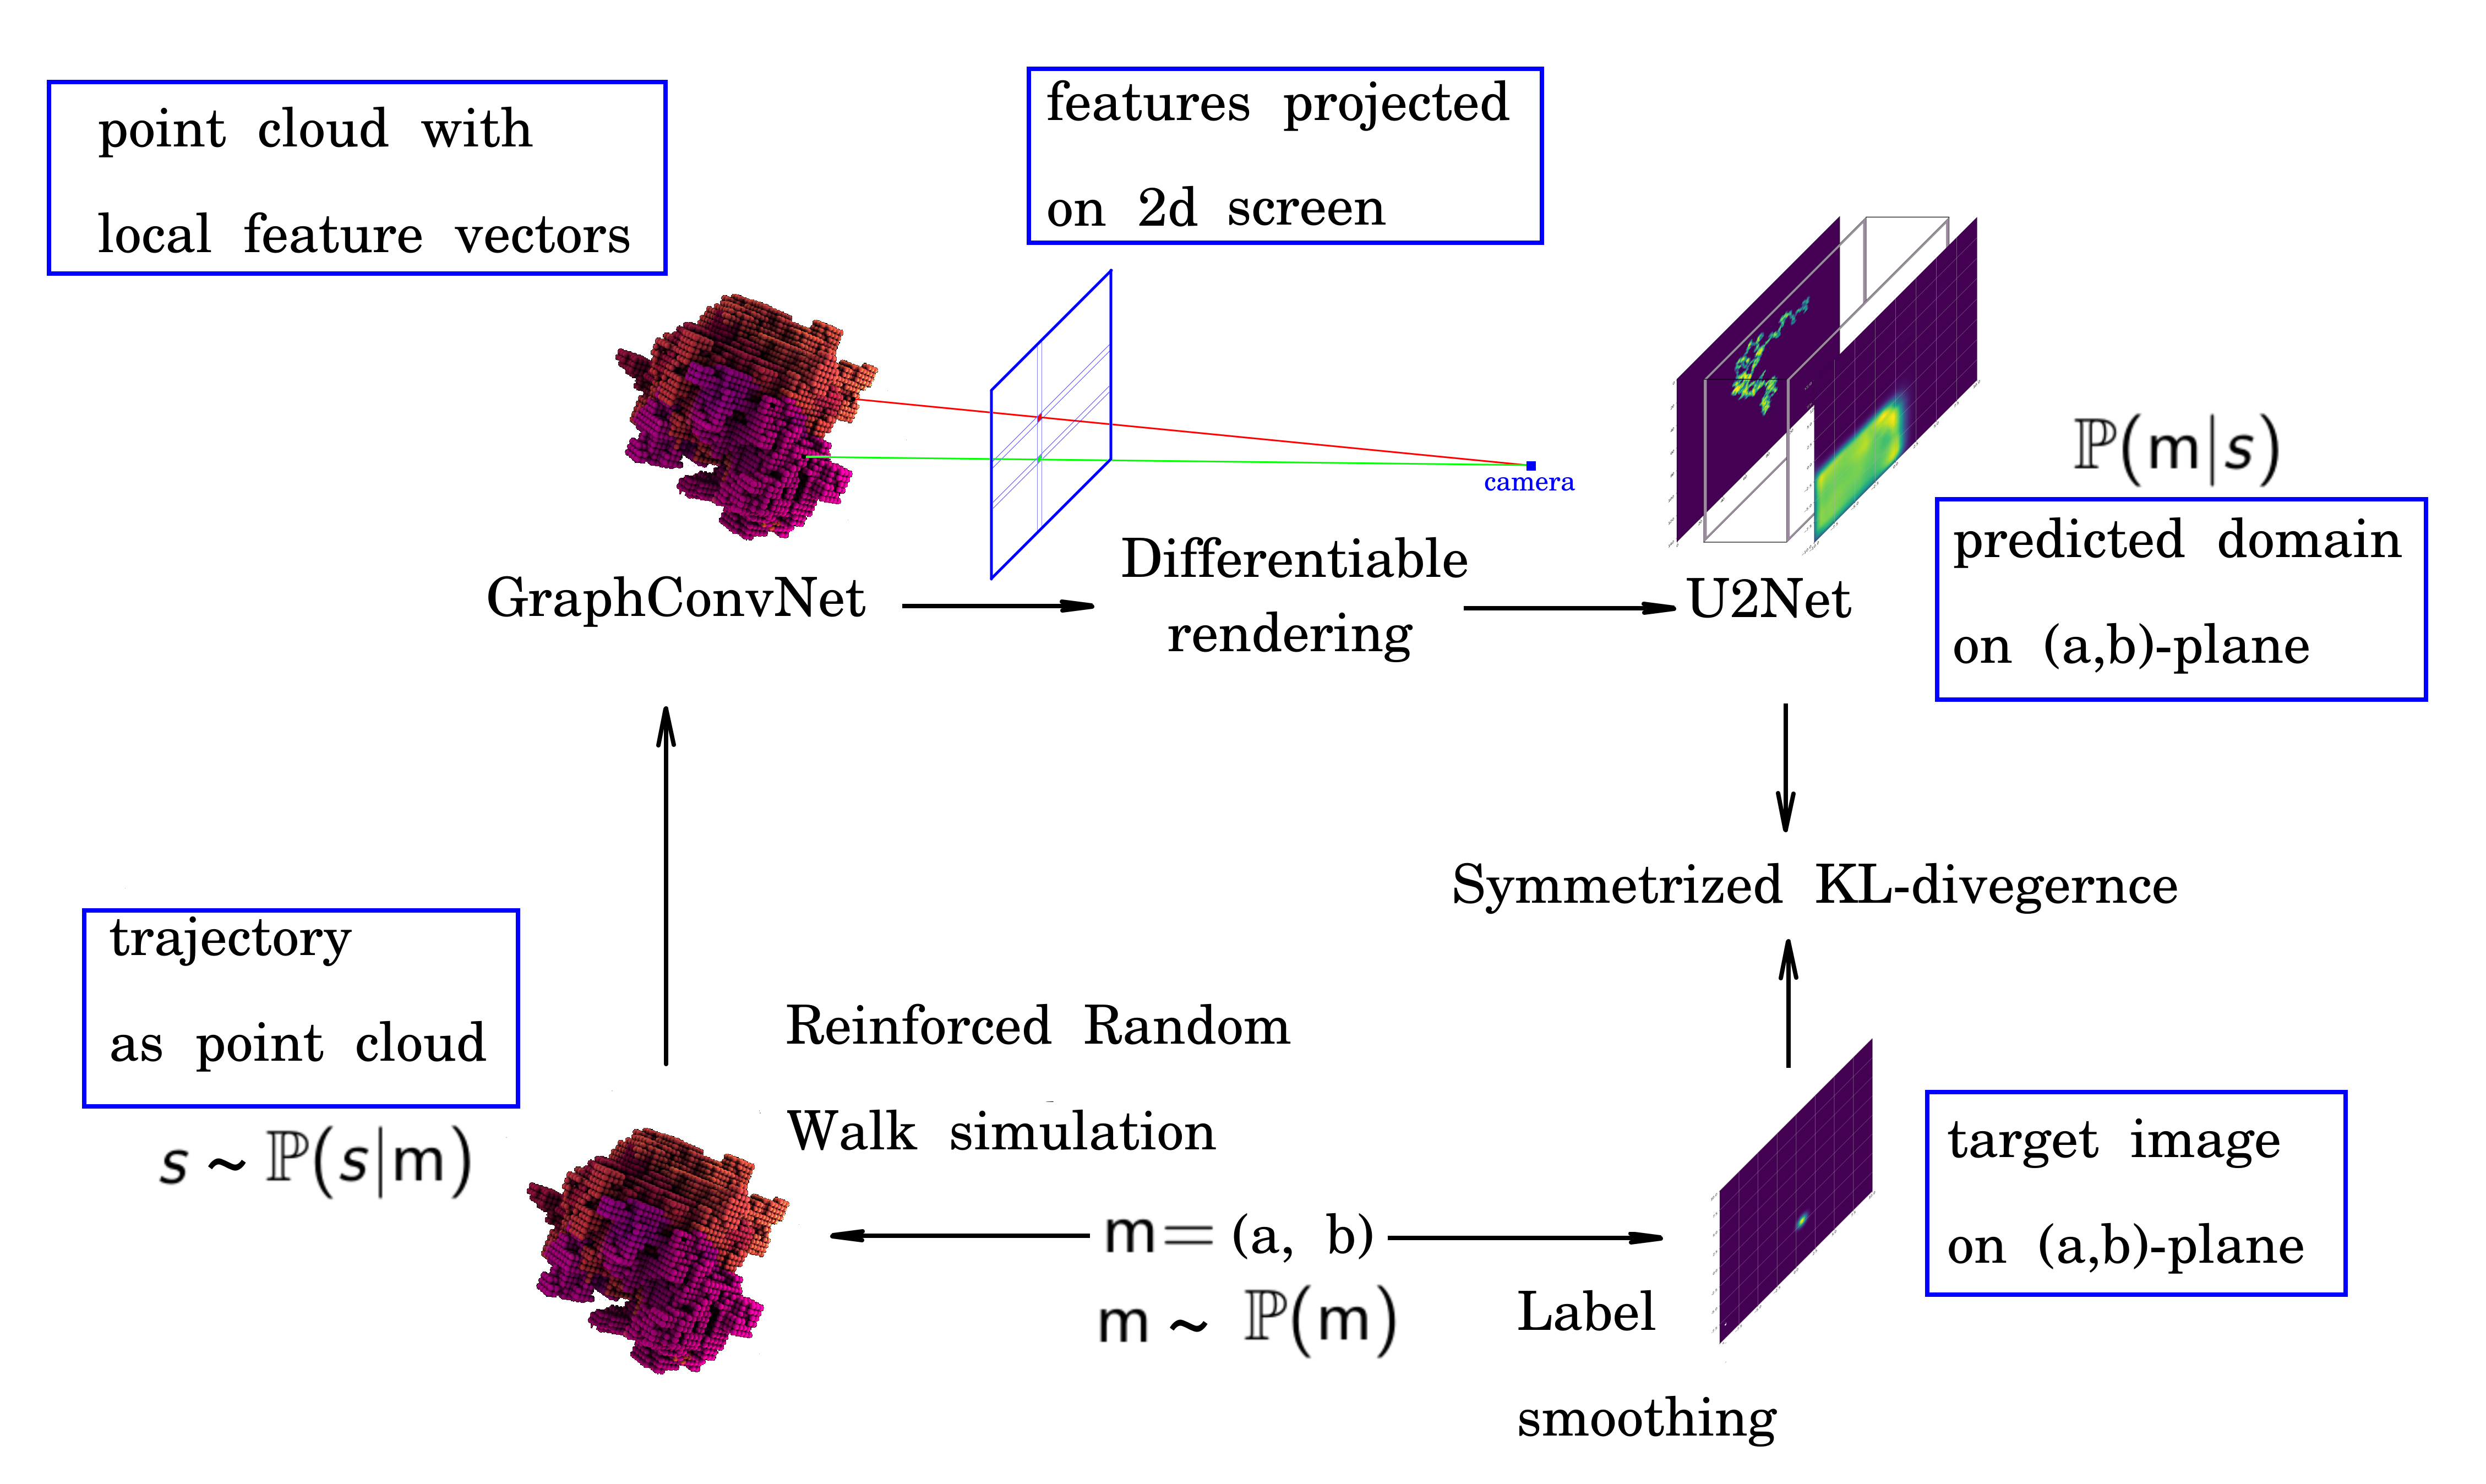
\includegraphics[width=8cm]{Fig1_rrw_analysis_scheme (2) (1).png}
\caption{General architecture of our machine learning approach.}
\label{scheme}
\end{figure}

% 
The main idea of our approach is as follows. Take a pair of parameters $(a,b)$ and generate a sufficiently long trajectory of a reinforced random walk with these parameters (we stop the trajectory generation when it has visited $N = 10^4$ distinct points). Then train a neural network to solve inverse problem of prediction possible values of macroscopic parameters for which a given trajectory could be generated. In contrast to previous approaches, instead of trying to predict exact values of parameters we rather estimate probability distribution on a space of macroscopic parameters. To achieve it we define target probability distribution as a smoothed Gaussian function centered at $(a,b)$. The idea is that, since two trajectories belonging to the same morphological phase are impossible to distinguish, the best neural network can do in order to predict $(a,b)$ is to highlight the whole range of possible parameters for which a given trajectory could have been obtained. To encode volumetric information we introduce a pipeline consisting of a graph convolutional network aggregating local features of point neighborhood and rasterization procedure projecting learned feature vectors on a 2d image. These images are processed by convolutional network based on $\text{U}^{2}$-Net architecture with output representing a probability distribution at predefined grid points in parameters space.

We are interested in reconstructing phase diagram of the model in a parameters region $\Omega$ from ensemble of microstates sampled uniformly inside $\Omega$. Define a grid in parameters space as  
$(a_{n}, b_{m}) = (a_{\text{min}} + \Delta a \cdot n, b_{\text{min}} + \Delta b \cdot m), \ n, m = 1, \dots, N.$ For a point $(\hat{a}, \hat{b}) \in \Omega$ target probability distribution encodes as $N \times N$ matrix is represented as 
$$
T_{m, n} = \frac{1}{2 \pi \sigma^{2}}\exp\left[-\frac{(\hat{a} - a_{n})^{2}+(\hat{b} - b_{m})^{2}}{2\sigma^{2}}\right]
$$

The main idea of our approach is as follows. Take a pair of parameters $(a,b)$ and generate a sufficiently long trajectory of a reinforced random walk with these parameters (we stop the trajectory generation when it has visited $N = 10^4$ distinct points, see \cite{supp} for details). Now, take an image of this trajectory (a photo taken from a random angle) and predict, based on it, the possible range of parameters for which it was generated. For that purpose we simultaneously train two neural networks: one takes a photo of the trajectory and transforms it into a non-negative function defined over $(a,b)$ plane; another takes the pair of initial parameters $(a,b)$ and produces a smoothed Gaussian function centered at $(a,b)$. The networks are trained in a way to make their outputs as close as possible. \fig{scheme} shows the outline of the classification scheme. The idea is that, since two trajectories belonging to the same morphological phase are impossible to distinguish, the best neural network can do in order to predict $(a,b)$ is to highlight the whole range of possible parameters for which a given trajectory could have been obtained. The label smoothing network (LS), which is needed in order to prevent divergence in the loss function is a 4-layered perceptron with 32 neurons in each layer. The detailed architecture of the image-analyzing network $\text{U}^{2}$-Net is given in \cite{supp} and the overall loss function for a given set of trajectory $\ve X$ and parameters $a,b$ reads
\be
\begin{array}{rll}
\mathcal{L}(\ve X, a,b) & = & \lambda \det(\text{cov}(\text{LS}(a,b)))^{2} + \medskip \\
& + & \displaystyle \sum_{\text{pixel-wise}} (\text{U}^{2}\text{Net}(\ve X)- \text{LS}(a,b))^{2}
\end{array}
\label{loss_v1}
\ee
where $\text{cov}(\text{LS}(a,b))$ is the covariance matrix of the Gaussian function, which is the output of the LS. The first term in \eq{loss_v1} is needed to prevent convergence of the output of both networks to a delocalized flat distribution. The detailed network training procedure is described in \cite{supp}. \fig{fig02} presents examples of the output of the networks. It is clearly seen that $\text{U}^{2}$-Net indeed produces as its output some clearly defined regions in the parameter space. 

\begin{figure}[ht]
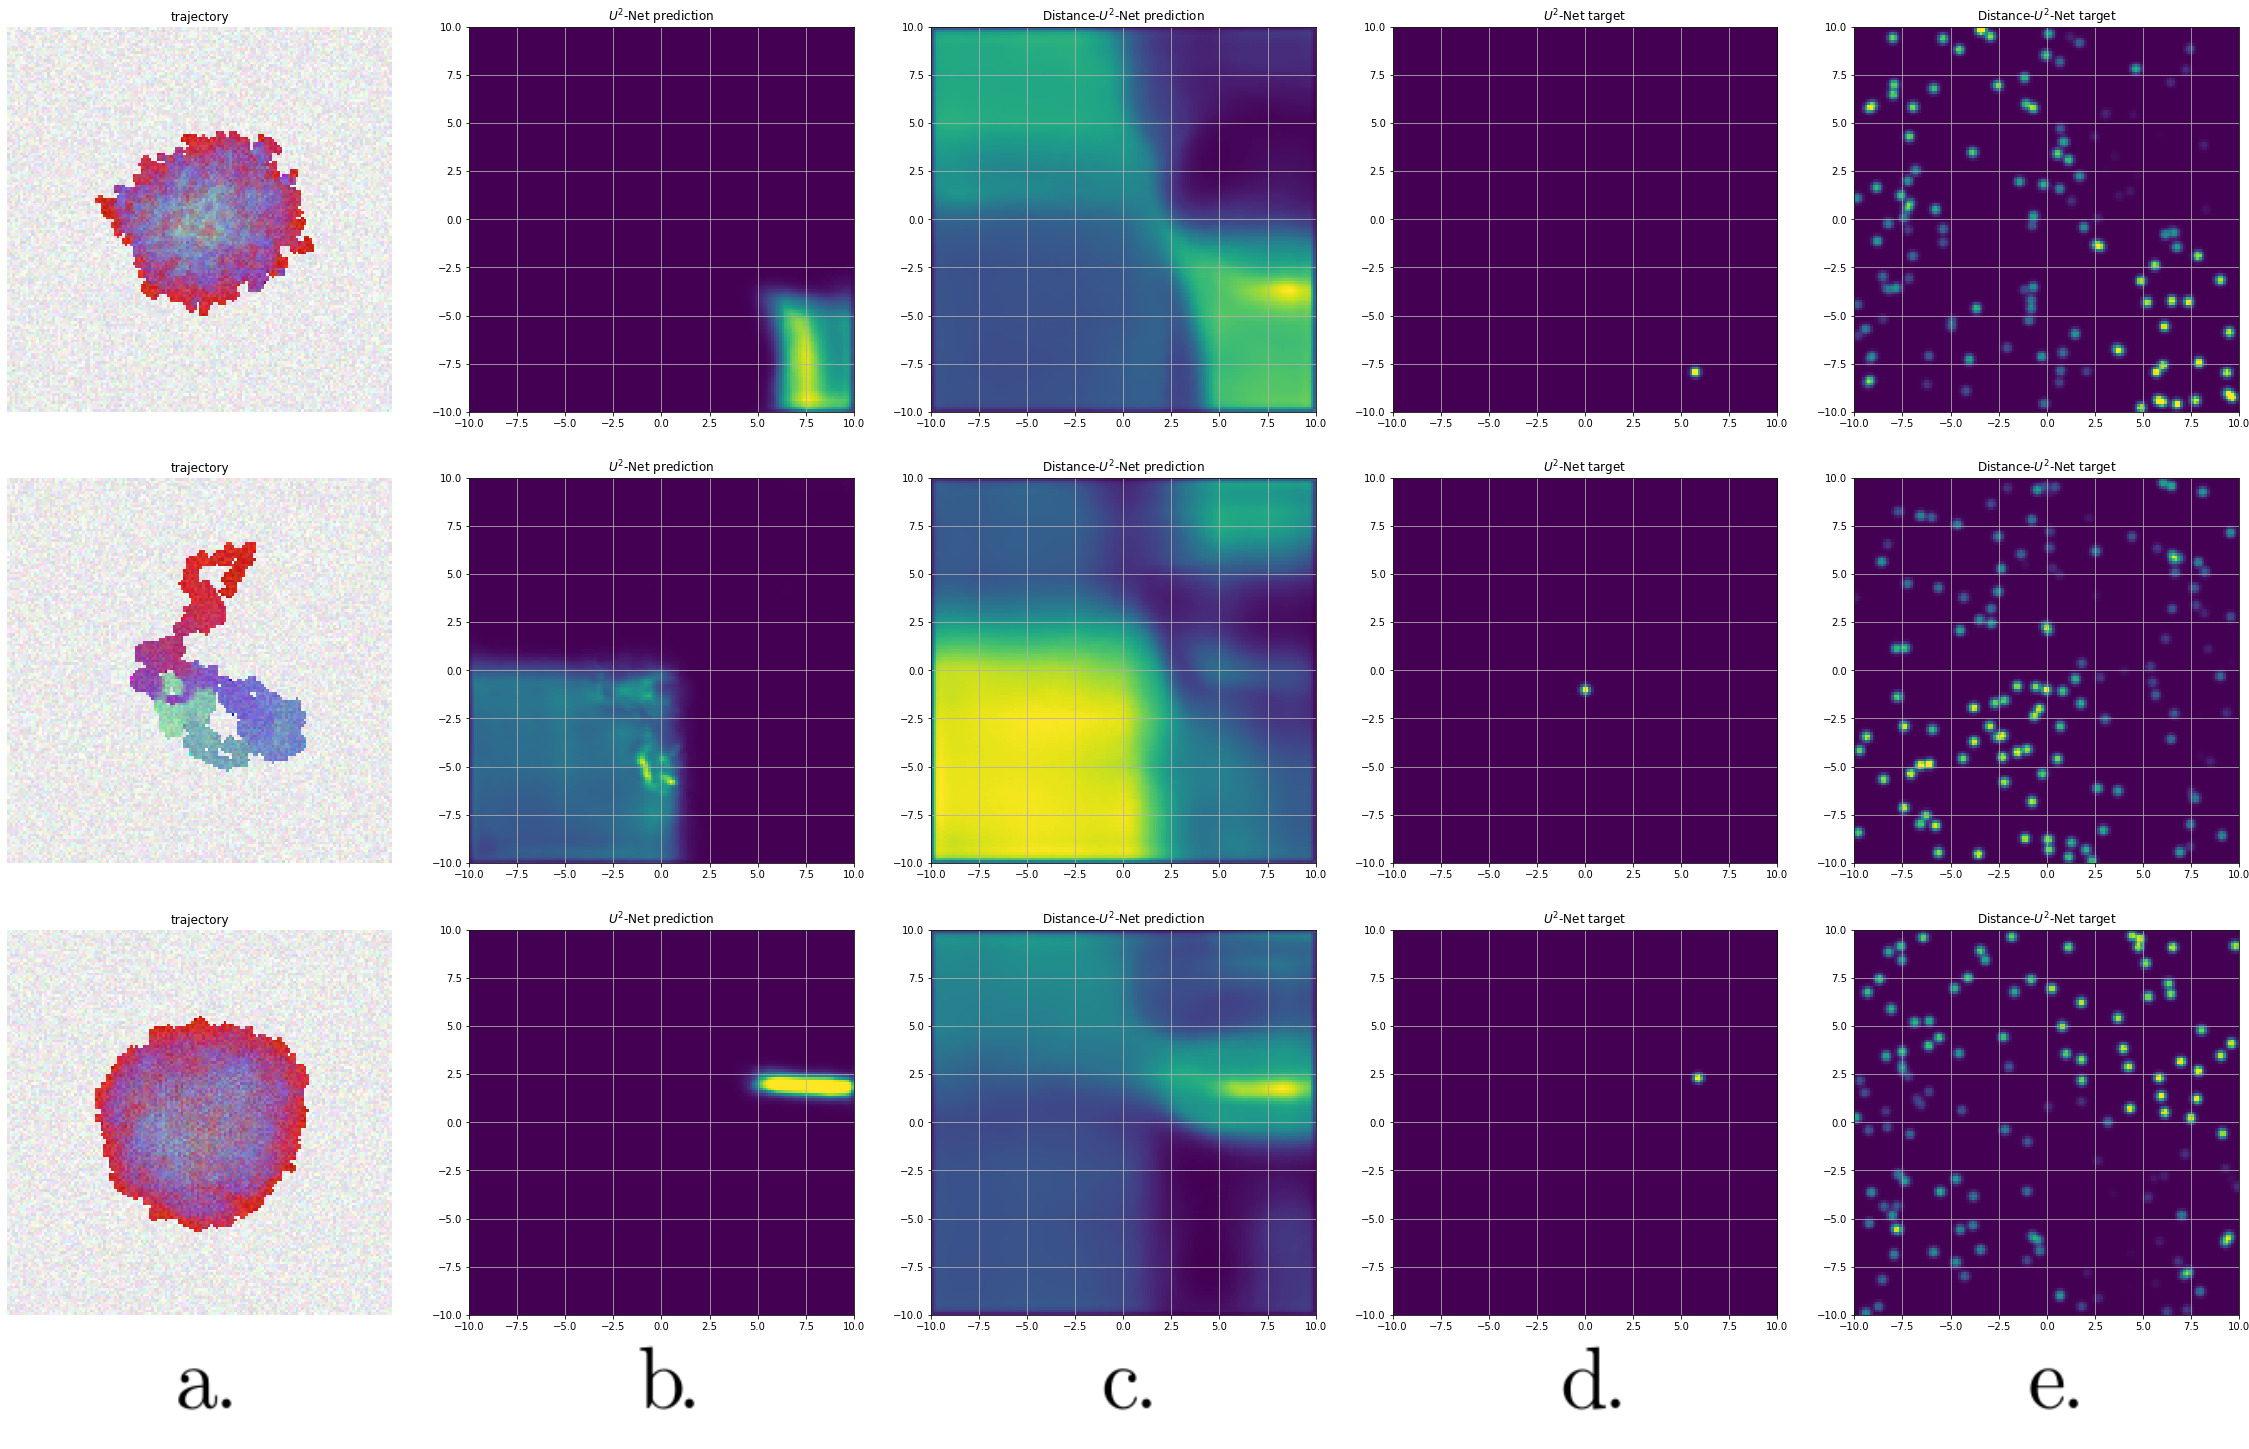
\includegraphics[width=8cm]{Fig2_input_output_example.png}
\caption{(a) Input of the first neural network: photo of a sample trajectory for $a =..., b = ...$ (top), $a =..., b = ...$ (bottom); (b) Output of a second neural network blurred point on the $(a,b)$ plane; (c) the output of a second neural network: network's estimate of possible $(a,b)$ region which might have generated the sample trajectory.}
\label{fig02}
\end{figure}

Given the output of $\text{U}^{2}$-Net, one can define a distance between two trajectories $\ve X$ and $\ve Y$ as follows
\be
\displaystyle d(\ve X, \ve Y) =  \frac{\sum_{\text{pixel-wise}}\left(\text{U}^{2}\text{Net}(\ve X)-\text{U}^{2}\text{Net}(\ve Y)\right)^2}{\sum_{\text{pixel-wise}}\left(\text{U}^{2}\text{Net}(\ve X)+\text{U}^{2}\text{Net}(\ve Y)\right)^2}
\label{distance}
\ee
Clearly, $d(\ve X, \ve Y)$ takes values between 0 and 1. Distance close to 0 corresponds to two trajectories generating a very similar output of $\text{U}^{2}$-Net, that is to say, areas on the $(a,b)$ plane, which strongly overlap. In turn, distance close to 1 means that wherever output $\text{U}^{2}\text{Net}(\ve X)$ differs from 0, the output $\text{U}^{2}\text{Net}(\ve Y)$ is essentially zero and vice versa. Therefore, distance defined above can work as an indicator of whether trajectories $\ve X$ and $\ve Y$ correspond to the same phase ($d(\ve X, \ve Y)\approx 1$) or to different phases  ($d(\ve X, \ve Y)\approx 0$). 

\begin{figure}[ht]
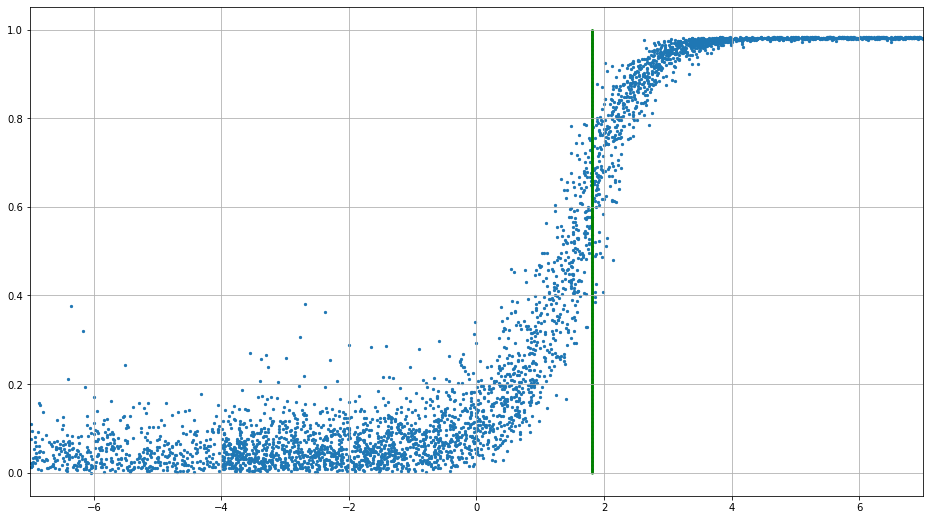
\includegraphics[width=8cm]{Fig3_reproduction_of_foster_results_for_phase_transition.png}
\caption{U-Net distance \eq{distance} from a Brownian motion trajectory ($a=-6, b=0$) to sample trajectories for $b=0$. Vertical green line corresponds to the transition point $a \approx 1.831$ found by finite-size scaling in \cite{ordemann1}.}
\label{fig03}
\end{figure}

In order to check whether the resulting classification is reasonable, we look at the particular case of $b=0$, which corresponds to volume-only reinforcement studied previously in \cite{sapozhnikov, ordemann1, ordemann2,foster}. Consider trajectories generated with $b=0$ and various $a$ and study their distance \eq{distance} from the trajectory generated at $a=-6,b=0$, i.e. deep within the true self-avoiding walk \cite{amit_parisi_peliti83} region. The results are shown in \fig{fig03}. One clearly sees a well-defined transition from trajectories similar to true self-avoiding walk to some different phase (the visited regions in this latter phase are known to be the asymptotically spherical and supercollapsed \cite{sapozhnikov, ordemann1}). The transition point as defined by the inflection point of the S-shaped curve in \fig{fig03} seems to be extremely close to $a_{cr} \approx 1.831$ found in  \cite{ordemann1} by finite-size scaling based on the statistics of much longer (up to $10^7$ steps) trajectories.   

The quality of the output may be further improved by a following trick.  Take a batch of 512 trajectories for randomly chosen values of $(a,b)$ and for each trajectory $\ve X_0 (a_0,b_0)$ in the batch find 15 closest trajectories $\ve X_i, \, i=1,\dots 15$ in the sense of \eq{distance}. Now, train network Dist-$\text{U}^{2}$-Net which has exactly the same architecture as $\text{U}^{2}$-Net to predict not just values of $(a_0,b_0)$ but also those of all 15 $(a_i,b_i)$ used to generating the trajectory $\ve X_i$. That is to say, to train the network Dist-$\text{U}^{2}$-Net we use a loss function  
\be
\begin{array}{rll}
 \mathcal{L}_2(\ve X) & = & \displaystyle \lambda \sum_{i=0..15} \det(\text{cov}(\text{LS}(a_i,b_i)))^{2} + \medskip \\
& + & \displaystyle \sum_{\text{pixel-wise}} \left(\text{Dist-U}^{2}\text{Net}(\ve X)- \sum_{i=0..15}\text{LS}(a_i,b_i)\right)^{2}
\end{array}
\label{loss}
\ee
As seen in Figure .. of \cite{supp}, the output of Dist-$\text{U}^{2}$-Net is similar to the output of $\text{U}^{2}$-Net but is much more uniform and has clearer boundaries. Thus, the network Dist-$\text{U}^{2}$-Net effectively separates the $(a,b)$ plane into non-intersecting regions which we classify as phases.   

\begin{figure}[ht]
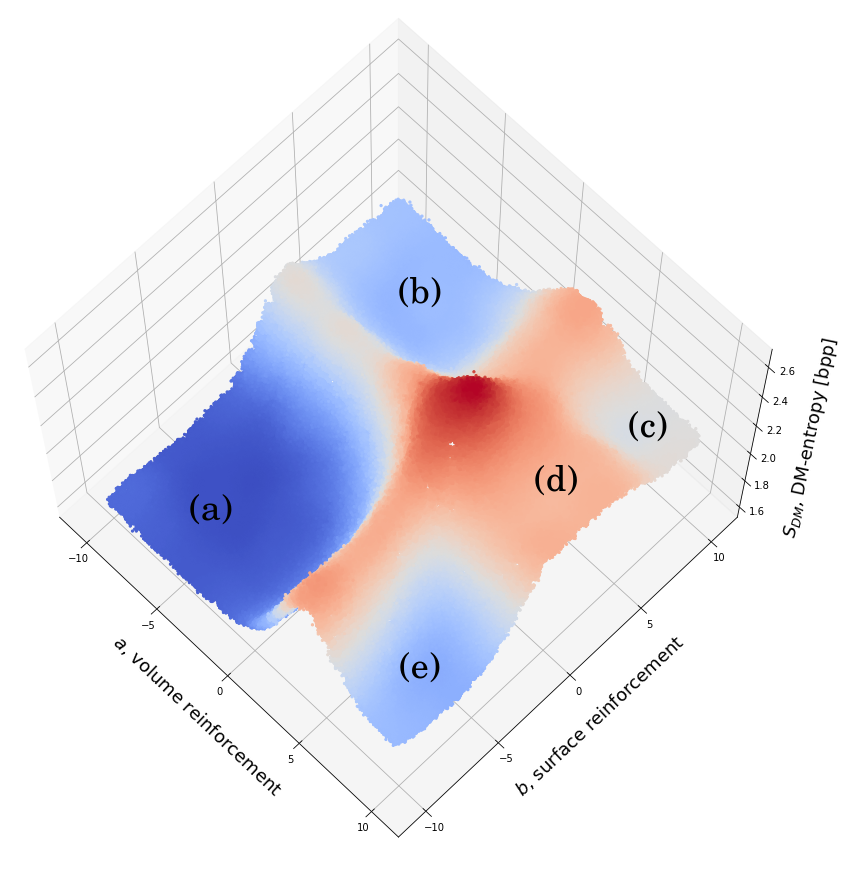
\includegraphics[width=8cm]{Effective_entropy (1).png}
\caption{Distance-map entropy of the model in the $(a,b)$ plane.}
\label{fig04}
\end{figure}

Direct inspection of the output shows that there are 5 distinct outputs corresponding to 5 distinct morphologies. In order to present the resulting phase diagram we clustered the output of the neural network into 5 clusters (see \cite{supp} for the details of the procedure). In \fig{fig04} we present the results of this clustering. Here dark blue regions correspond to such values of parameters for which corresponding trajectories are always classified into the same cluster, i.e. these parameters reliably belong inside a phase, rather than on a phase boundary. In turn, trajectories corresponding to the points in the light blue regions are, depending on the realization, classified into one of two clusters, meaning that they are in the vicinity of a transition line between two phases. Finally, trajectories corresponding to the yellow regions got classified into three or more different clusters, outlining the vicinity of triple points on the phase diagram. 

\begin{figure}[ht]
\includegraphics[width=8.8cm]{Fig5_trajectories_large.png}
\caption{Examples of representative trajectories of the 5 phases found in a phase diagram.}
\label{fig05}
\end{figure}

In \fig{fig05} we show the examples of morphologies corresponding to the 5 regions in the phase diagram. Phase (a) is a simple Brownian motion or true self-avoiding walk with spatial extension of $N$-step walk proportional to $N^{1/2}$ and Gaussian distribution of the end-to-end distance. Phase (d) is the phase of supercollapsed ball first predicted in \cite{sapozhnikov} and well-studied in the volume-reinforced ($b=0$) case. The visited region of the walk is in this case asymptotically a smooth ball with radius growing as $N^{1/4}$ with growing number of steps. 

Phase (c), first conjectured in \cite{kot_phase}, is similar to phase $d$ but for the fact that the supercollapsed ball in this case has a rough surface and is porous. As a result, the surface and the volume of the ball are growing as $N^{2\sigma}$ and $N^{3\nu}$, respectively, with $\sigma>\nu$. There is an easy scaling argument establishing connection between $\sigma$ and $\nu$. Indeed, in the $e^a\gg \max(1, e^b)$ limit the walk spends most of the time inside the already visited volume, whose surface almost always reflects it. As a result, the probability of finding walker in any point inside the visited volume is the same (more precisely, converges to uniform distribution after many reflections from the boundary). If the walker is currently at the surface of the visited volume he has some small probability to go outside and thus increase the visited volume by one new lattice cite. If it is not on the surface (i.e., in the inner part of the visited volume), then the probability of increasing volume on the next step is zero. Thus,
\be
\frac{dV}{dN} = const \times \frac{S}{V}; \;\; \rightarrow \;\; 6\nu  = 1+2\sigma,
\label{scaling}
\ee 
where constant depends on the particular values of $a$ and $b$. In the case of phase (d) the exponents $\sigma$ and $\nu$ are the same, which leads to $\nu =1/4$ \cite{sapozhnikov}. For phase (c) the exact values of $\nu$ and $\sigma$ are unknown, and it is not even clear if they are constant throughout the phase or change with $a$ and $b$. 

In phase (b) the walk is mostly sticking to the surface of the already visited region, without either penetrating it or going away. As a result, visited volume grows, at least approximately, proportionally to the number of steps but the visited area forms a rather irregularly shaped blob (see \fig{fig05}:b) with a very developed surface, which is reminiscent of the shapes of polymer rings in a melt \cite{grosb_review,rosa_everaers} (see also supplementary materials of \cite{tamm15} where a very similar construction was used to generate approximate initial condition for a crumpled chromatin-like polymer). 

To understand phase (e) note that on the $a,b \gg 1$ limit it is beneficial for the visited volume to have extended flat faces, which grow without defects up to the area of order $e^b$. As a result, crystalline-like objects like one shown in \fig{fig05}:e are formed. Clearly, for any given $a,b$ they are unstable in the $N \to \infty$ limit, but the length of the walk needed for the defects to destroy this crystalline structure is exponentially large. However, the existence of this phase is a peculiarity of the simple cubic lattice, which is conducive to the flat face formation. In \cite{supp} we check that phase diagram of a similar walk on body-centered cubic lattice does not include this phase. Instead, there is a direct transition from crumpled-globule-like phase (b) to supercondensed ball phase (d).


{\it Here will be a discussion}

The authors are grateful to L. Nazarov and N. Kotelevskii who contributed to preliminary numerical analysis of the reinforced random walk model by means of direct Monte Carlo simulations. This research was supported in part through computational resources of HPC facilities at
NRU HSE and by BASIS Foundation grants 17-12-278-1 and 19-1-1-48-1.

\begin{thebibliography}{99}

\cite{phase_transitions_by_confusion, carrasquilla, ml_topological_phase_transitions, ml_quantum_phase_transitions, ml_hubbard_model, pca_and_vae_ising_model}

\bibitem{phase_transitions_by_confusion} Van Nieuwenburg, E. P., Liu, Y. H., & Huber, S. D. (2017). Learning phase transitions by confusion. Nature Physics, 13(5), 435-439.

\bibitem{carrasquilla} Carrasquilla, J., & Melko, R. G. (2017). Machine learning phases of matter. Nature Physics, 13(5), 431-434.

\bibitem{ml_topological_phase_transitions} Rodriguez-Nieva, J. F., & Scheurer, M. S. (2019). Identifying topological order through unsupervised machine learning. Nature Physics, 15(8), 790-795.

\bibitem{ml_quantum_phase_transitions} Rem, B. S., Käming, N., Tarnowski, M., Asteria, L., Fläschner, N., Becker, C., ... & Weitenberg, C. (2019). Identifying quantum phase transitions using artificial neural networks on experimental data. Nature Physics, 15(9), 917-920.

\bibitem{ml_hubbard_model} Bohrdt, A., Chiu, C. S., Ji, G., Xu, M., Greif, D., Greiner, M., ... & Knap, M. (2019). Classifying snapshots of the doped Hubbard model with machine learning. Nature Physics, 15(9), 921-924.

\bibitem{pca_and_vae_ising_model} Wetzel, S. J. (2017). Unsupervised learning of phase transitions: From principal component analysis to variational autoencoders. Physical Review E, 96(2), 022140.



\bibitem{Van_Nieuwenburg} Van Nieuwenburg, Evert PL, Ye-Hua Liu, and Sebastian D. Huber. "Learning phase transitions by confusion." Nature Physics 13.5 (2017): 435-439.

\bibitem{sapozhnikov} Sapozhnikov, Victor B. "Self-attracting walk with $\nu< 1/2$." Journal of Physics A: Mathematical and General 27.6 (1994): L151.

\bibitem{ordemann1} A. Ordemann, G. Berkolaiko, S. Havlin , and A. Bunde, Swelling-Collapse Transition of Self-Attracting Walks, Physical Review E, V. 61, N 2, P. 1005-1007 (2000).

\bibitem{ordemann2} A. Ordemann, E. Tomer, G. Berkolaiko, S. Havlin, and A. Bunde, Structural Properties of Self-Attracting Walks, Physical Review E, V. 64, 046117 (2001).

\bibitem{foster} Foster, Jacob G., Peter Grassberger, and Maya Paczuski. "Reinforced walks in two and three dimensions." New Journal of Physics 11.2 (2009): 023009.

\bibitem{grover} Grover, A., & Leskovec, J. (2016, August). node2vec: Scalable feature learning for networks. In Proceedings of the 22nd ACM SIGKDD international conference on Knowledge discovery and data mining (pp. 855-864).

\bibitem{BhatRednerBenichou17} Bhat, S. Redner, O. Benichou, 2017.

\bibitem{amit_parisi_peliti83} Parisi, Peliti, 1983.

\bibitem{gns88} A.Yu. Grosberg, S. Nechaev, E. Shakhnovich, J. de Physique, 1988.

\bibitem{grosberg93} A.Yu. Grosberg, S. Havlin, et al., 1993.

\bibitem{mirny09} L. Mirny, Chromosome Res., 2009.

\bibitem{tamm15} M.V. Tamm, L.I. Nazarov, A.A. Gavrilov, A.V. Chertovich, "Anomalous diffusion in fractal globules." Physical review letters 114.17 (2015): 178102.

\bibitem{supp} A. Lobashev, S. Nechaev, M. Tamm, supplementary materials to this paper.

\bibitem{kot_phase} N.Y. Kotelevskii, S.K. Nechaev, M.V. Tamm, ``A new class of reinforced random walks'', Book of Abstracts of ``International Conference on Computer Simulation in Physics and beyond'', p. 138, Moscow, 2018. 

\bibitem{rosa_everaers} Everaers,  Rosa, Grosberg  Rings

\bibitem{grosb_review} Smrek, Halverson, Kremer, Grosberg, Review



\bibitem{original_pixelcnn} Van Oord, A., Kalchbrenner, N., & Kavukcuoglu, K. (2016, June). Pixel recurrent neural networks. In International Conference on Machine Learning (pp. 1747-1756). PMLR.

\bibitem{conditional_pixelcnn}  Oord, A. V. D., Kalchbrenner, N., Vinyals, O., Espeholt, L., Graves, A., & Kavukcuoglu, K. (2016). Conditional image generation with pixelcnn decoders. arXiv preprint arXiv:1606.05328.

\bibitem{locally_masked_pixelcnn} Jain, A., Abbeel, P., & Pathak, D. (2020, August). Locally Masked Convolution for Autoregressive Models. In Conference on Uncertainty in Artificial Intelligence (pp. 1358-1367). PMLR.

\bibitem{arnold} Arnol'd, V. I. (2013). Mathematical methods of classical mechanics (Vol. 60). Springer Science & Business Media.

\bibitem{arnold_khesin} Arnold, V. I., & Khesin, B. A. (1998). Topological methods in hydrodynamics (Vol. 125, pp. 69-73). New York: springer.

\bibitem{sardanashvily_0} Sardanashvily, G.A. (2011). Modern Methods of Field Theory.

\bibitem{sardanashvily_1} Sardanashvily, G. (2008). Classical Field Theory: Advanced Mathematical Formulation. International Journal of Geometric Methods in Modern Physics, 5(07), 1163-1189.

\bibitem{sardanashvily_2} Sardanashvily, G. (1992). On the geometry of spontaneous symmetry breaking. Journal of Mathematical Physics, 33(4), 1546-1549.

\bibitem{sardanashvily_3} Mangiarotti, L., & Sardanashvily, G. A. (2000). Connections in classical and quantum field theory. World Scientific.

\bibitem{eberard} Eberard, D., Maschke, B. M., & Van Der Schaft, A. J. (2007). An extension of Hamiltonian systems to the thermodynamic phase space: Towards a geometry of nonreversible processes. Reports on mathematical physics, 60(2), 175-198.

\bibitem{bravetti_1} Bravetti, A. (2017). Contact Hamiltonian dynamics: The concept and its use. Entropy, 19(10), 535.

\bibitem{bravetti_2} Bravetti, A. (2019). Contact geometry and thermodynamics. International Journal of Geometric Methods in Modern Physics, 16(supp01), 1940003.

\bibitem{caratheodory} Carathéodory, C. (1909). Untersuchungen über die Grundlagen der Thermodynamik. Mathematische Annalen, 67(3), 355-386.

\bibitem{goto} Goto, S. I. (2015). Legendre submanifolds in contact manifolds as attractors and geometric nonequilibrium thermodynamics. Journal of Mathematical Physics, 56(7), 073301.

\bibitem{wasserstein_distance} Kantorovich, L., Rubinstein, G. (1958). On a space of completely additive functions. Vestn. Leningr. Univ. Math. 13, 7, 52-59.

\bibitem{sapozhnikov} Sapozhnikov, V. B. (1994). Self-attracting walk with $\nu<1/2$. Journal of Physics A: Mathematical and General, 27(6), L151.

\bibitem{ordemann_1} Ordemann, A., Berkolaiko, G., Havlin, S., & Bunde, A. (2000). Swelling-collapse transition of self-attracting walks. Physical Review E, 61(2), R1005.

\bibitem{ordemann_2} Ordemann, A., Tomer, E., Berkolaiko, G., Havlin, S., & Bunde, A. (2001). Structural properties of self-attracting walks. Physical Review E, 64(4), 046117.

\bibitem{foster} Foster, J. G., Grassberger, P., & Paczuski, M. (2009). Reinforced walks in two and three dimensions. New Journal of Physics, 11(2), 023009.

\bibitem{true_saw} Amit, D. J., Parisi, G., & Peliti, L. (1983). Asymptotic behavior of the" true" self-avoiding walk. Physical Review B, 27(3), 1635.

\bibitem{grover} Grover, A., & Leskovec, J. (2016, August). node2vec: Scalable feature learning for networks. In Proceedings of the 22nd ACM SIGKDD international conference on Knowledge discovery and data mining (pp. 855-864).

\bibitem{melt_of_rings_crumpling} Rosa, A., & Everaers, R. (2014). Ring polymers in the melt state: the physics of crumpling. Physical review letters, 112(11), 118302.

\bibitem{melt_of_rings_chromosomes} Halverson, J. D., Smrek, J., Kremer, K., & Grosberg, A. Y. (2014). From a melt of rings to chromosome territories: the role of topological constraints in genome folding. Reports on Progress in Physics, 77(2), 022601.

\bibitem{nazarov_tamm} Tamm, M. V., Nazarov, L. I., Gavrilov, A. A., & Chertovich, A. V. (2015). Anomalous diffusion in fractal globules. Physical review letters, 114(17), 178102.

\bibitem{u2net} Qin, X., Zhang, Z., Huang, C., Dehghan, M., Zaiane, O. R., & Jagersand, M. (2020). U2-Net: Going deeper with nested U-structure for salient object detection. Pattern Recognition, 106, 107404.

\bibitem{lobashev_1} A. Lobashev. (2020, October). Surface and Volume Reinforced Random Walk, International Conference on Computer Simulation in Physics and beyond.

\bibitem{lobashev_2} A. Lobashev, M. Tamm. (2020, December).  Contrastive Learning Approach for Phase Diagram Construction of the Random Walk Model with Volume and Surface Reinforcement, Conference on Complex Systems 2020.

\bibitem{lobashev_3} A. Lobashev, M. Tamm. (2021, May). Conformational Entropy Estimation of a Non-Markovian Random Walk by Autoregressive Generative Modeling, The 46th Conference of the Middle European Cooperation in Statistical Physics.

\end{thebibliography}

\end{document}